\documentclass[11pt]{article}

\usepackage[margin=1in]{geometry}
\usepackage{graphicx}
\usepackage{booktabs}
\usepackage{amsmath}
\usepackage{amssymb}
\usepackage{caption}
\usepackage[hidelinks]{hyperref}
\usepackage{times}

\setlength{\parindent}{0pt}
\setlength{\parskip}{0.72em}
\captionsetup{font=small,labelfont=bf,skip=4pt}
\renewcommand{\arraystretch}{1.08}
\renewcommand{\topfraction}{0.92}
\renewcommand{\bottomfraction}{0.85}
\renewcommand{\textfraction}{0.06}
\renewcommand{\floatpagefraction}{0.80}

\title{\vspace{-2em}When the Budget Is Actually Spent:\\
Forced Reasoning Depth against Agents, Rounds, and Sampling}
\author{Study \texttt{openrouter\_forced\_budget\_v2}}
\date{18 September 2026}

\begin{document}
\maketitle
\vspace{-1.5em}

\section*{Abstract}

A fixed inference budget can buy more agents, more rounds of revision, more independent samples read
out by a vote, or a longer chain of reasoning inside a single call. The first study in this series
(v1, \texttt{openrouter\_agent\_\allowbreak allocation\_v1}) compared these at a nominal budget $C = B \cdot R \cdot A$ and
found that allocation shape barely mattered. It had a flaw that this study removes: the per-call
reasoning allowance $A$ was a cap the model was free to leave unspent, and it did. A single call allowed
{{v1_deep.16.requested|d}} reasoning tokens spent {{v1_deep.16.realized|d}}, so ``depth'' was never
actually bought.

Here every generation is forced to spend exactly its budget. Over OpenRouter's raw completion endpoint the
end-of-reasoning token is banned with a logit bias until the budget is exhausted, and a second call reads
the model's own reasoning back to write the answer; the model sees one prompt and no injected text. All
{{n_generations_main|d}} main-run generations realized exactly their budget. The study ran the full v1 grid
of {{n_checkpoints_ladder|d}} configurations on Qwen3.8-27B, over {{n_items|d}} items from four hard
benchmarks (AIME 2025 and 2026, HMMT February 2025 and 2026, Omni-MATH at difficulty 7 and above,
GPQA-Diamond), at $A = 1024$ tokens per call, for {{spend_all_usd|$}} of generation cost.

Once depth is real, allocation shape matters a great deal, and one direction dominates. A single call
forced to $16A$ delivers {{acc.macro.deep/16.acc|3}} on the four-benchmark macro, against
{{acc.macro.sample/16.acc|3}} for sixteen independent samples and a vote at the same realized compute,
a paired difference of {{depth_vs_width.macro.16.deep_minus_sample.pts|+1}} points
(95\% CI {{depth_vs_width.macro.16.deep_minus_sample.lo|+1}} to {{depth_vs_width.macro.16.deep_minus_sample.hi|+1}}).
It also exceeds oracle pass@16 of the same sampling bank by {{deep_vs_oracle.macro.16|1}} points: no
selector over sixteen short samples could have matched it. A call at $4A$ beats twenty-five samples
by {{cross.deep4_minus_sample25.macro.pts|1}} points. The best configuration without a deep call,
{{best.macro.non_deep_name|tt}}, reaches {{best.macro.non_deep_acc|3}}. Every point on the
accuracy-per-dollar frontier is a deep call.

The effect is carried by competition mathematics. On GPQA-Diamond depth and serial revision tie, and the
best configuration is a single agent revising its own answer. Sequential revision is the second-best
lever: a private revision chain is above sampling at every budget of three calls or more, significantly so at {{iso.macro.by_family.private_single.n_sig_pos|d}} of {{iso.macro.by_family.private_single.n|d}} budgets. Letting agents see
each other's work now helps slightly rather than hurting as it did in v1. The binding constraint in v1 was
selection; here it is the depth of a single chain of thought, which neither width nor a vote can supply.

\section{Methods}

\subsection{Why a second study}

In v1 the per-call reasoning allowance was a soft request to Gemini 2.5 Flash-Lite. Realized reasoning
flattened at a few thousand tokens however much was requested (Figure~\ref{fig:v1v2}a), so the
\texttt{deep}/$m$ family spent a fraction of its nominal budget and every iso-compute comparison involving
it compared unequal amounts of computation. v1's finding that ``one deep call matches the best
orchestration'' was therefore a statement about a call that was not deep. This study keeps v1's design,
protocols, prompts, selectors and estimators, and changes three things: the budget is enforced, the
model is an open-weight reasoning model whose decoding can be controlled, and the benchmarks are hard
enough that a forced budget cuts reasoning short rather than padding a finished answer.

\begin{figure}[htbp]
\centering
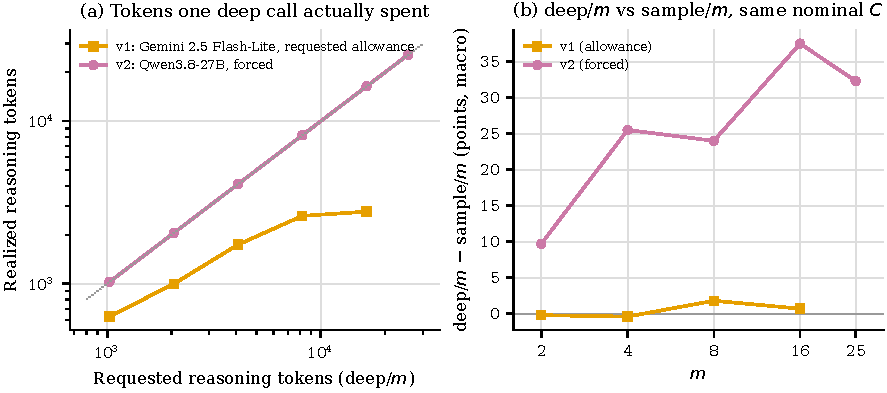
\includegraphics[width=\textwidth]{figures/f4_requested_vs_realized.pdf}
\caption{(a) Reasoning tokens one deep call actually spent against the tokens requested: v1 on its main
panel (Gemini 2.5 Flash-Lite, a soft allowance) and v2 (Qwen3.8-27B, forced). The dotted line is equality.
(b) The consequence for the headline comparison: deep/$m$ minus sample/$m$ on each study's macro. The
two studies differ in model and benchmarks, so (b) contrasts what each design could measure, not the same
quantity twice.}
\label{fig:v1v2}
\end{figure}

\subsection{Forcing the budget}

Each generation node is two calls to OpenRouter's \texttt{/completions} endpoint. The THINK call sends
the model's own chat template, rendered from the node's system and user messages and ending with an
opened reasoning block, with a logit bias of $-100$ on the end-of-reasoning token and the two
end-of-sequence tokens, and \texttt{max\_tokens} equal to the node's budget. The model therefore cannot
close its reasoning and the call ends exactly at the budget. The ANSWER call re-sends the same prompt,
the model's reasoning verbatim and the closing tag, and lets the model write its visible answer freely
under a 4096-token cap. The model is never shown a new instruction or any injected text; the only seam is
that the reasoning is re-tokenized, which adds two or three prompt tokens.

Many OpenRouter endpoints list \texttt{logit\_bias} as supported but silently ignore it, which a +100
bias on an ordinary word exposes at once. Every endpoint was screened this way before use, and each
dispatcher re-ran the screen (together with an exact-length forced call and an answer check) before any
paid work; the screen refused to dispatch into one transient provider outage during the pilot. A THINK
call that ends short of its budget, which happens when a provider cuts a stream, is treated as a
transport failure and retried, never counted. The {{retries.attempts|d}} retried attempts in the main run
cost {{retries.usd|$}}.

The result is exact: every one of the {{n_generations_main|d}} main-run generations realized exactly its
reasoning budget ({{forced_not_exact|d}} exceptions). The budget $C = B\cdot R\cdot A$
of every configuration below is therefore both requested and realized.

\subsection{Model, benchmarks and panels}

Generations come from \texttt{qwen/qwen3.8-27b} at the model's recommended sampling (temperature 1.0,
nucleus 0.95, top-$k$ 20), with the provider pinned per item, fallbacks disabled and response caching
off. Two providers served the run concurrently, each on its own disjoint set of items: Mancer
({{shard_items.mancer|d}} main items) and Parasail ({{shard_items.parasail|d}}). Because every item stays on
one provider, every within-item contrast is same-provider.

Four benchmarks are scored, {{n_items_by_bench.aime|d}} main items each: AIME 2025 and 2026 and HMMT
February 2025 and 2026 (graded by Math-Verify), Omni-MATH problems of difficulty 7 or more (Math-Verify,
with items whose gold answer is prose or unparseable excluded before any generation), and GPQA-Diamond
(four options shuffled once per item with a fixed seed, exact option match). The panel was drawn by the
harness's frozen, stratified procedure; no item was chosen by model performance.

A pre-registered calibration on eight development items per benchmark (disjoint from the main panel)
required forced pass@1 at $A=1024$ between 0.15 and 0.85 for each benchmark to stay; all four passed
(Table~\ref{tab:cal}). The same calibration ran one unforced generation per item, which shows the regime:
left to itself the model reasons for thousands to tens of thousands of tokens on these problems, so a
forced $A = 1024$ truncates each call hard, and the deep calls up to $25A$ mostly stay at or below the
length the model would choose.

\begin{table}[htbp]
\centering
\small
\begin{tabular}{lrrrr}
\toprule
Benchmark & forced pass@1 ($A$=1024) & natural pass@1 & natural reasoning, median & mean \\
\midrule
AIME 25+26 & {{calibration.aime.forced_pass_at_1|3}} & {{calibration.aime.natural_pass_at_1|3}} & {{calibration.aime.natural_reasoning_tokens_median|d}} & {{calibration.aime.natural_reasoning_tokens_mean|d}} \\
HMMT Feb 25+26 & {{calibration.hmmt.forced_pass_at_1|3}} & {{calibration.hmmt.natural_pass_at_1|3}} & {{calibration.hmmt.natural_reasoning_tokens_median|d}} & {{calibration.hmmt.natural_reasoning_tokens_mean|d}} \\
Omni-MATH $\geq$7 & {{calibration.omni_math_hard.forced_pass_at_1|3}} & {{calibration.omni_math_hard.natural_pass_at_1|3}} & {{calibration.omni_math_hard.natural_reasoning_tokens_median|d}} & {{calibration.omni_math_hard.natural_reasoning_tokens_mean|d}} \\
GPQA-Diamond & {{calibration.gpqa_diamond.forced_pass_at_1|3}} & {{calibration.gpqa_diamond.natural_pass_at_1|3}} & {{calibration.gpqa_diamond.natural_reasoning_tokens_median|d}} & {{calibration.gpqa_diamond.natural_reasoning_tokens_mean|d}} \\
\bottomrule
\end{tabular}
\caption{Calibration on 8 development items per benchmark (not the main panel). Natural generations were
capped at 25,600 reasoning plus 4,096 answer tokens; on Omni-MATH the median call reached that cap, so its
natural length is a lower bound.}
\label{tab:cal}
\end{table}

\subsection{The compute accounting}

Each configuration is a triple $(B, R, A)$ and its budget is their product, read from the sealed
tables rather than parsed from names:

\begin{center}
\small
\begin{tabular}{llccc}
\toprule
Family & Notation & $B$ & $R$ & $C$ \\
\midrule
Independent samples, plurality vote & \texttt{sample/k} & $k$ & 1 & $kA$ \\
One agent revising its own answer & \texttt{private\_single/t} & 1 & $t$ & $tA$ \\
Team, no peer exposure & \texttt{private\_team/n/r} & $n$ & $1+r$ & $n(1+r)A$ \\
Team, peer exposure & \texttt{peer/n/r} & $n$ & $1+r$ & $n(1+r)A$ \\
One deeper call & \texttt{deep/m} & 1 & 1 & $mA$ \\
\bottomrule
\end{tabular}
\end{center}

$A = 1024$ throughout, $m \in \{1,2,4,8,16,25\}$ (deep/25 is new, so that depth reaches the 25-generation
budgets), teams have $n \in \{2,\dots,5\}$ and $r \in \{1,\dots,4\}$, and deep/1 is root[0] of the
sampling bank. Figure~\ref{fig:design} shows the design: five budget levels ($C/A \in \{2,4,8,16,25\}$)
carry a deep call alongside several multi-call allocations, which is where depth and width meet at equal
realized compute.

\begin{figure}[htbp]
\centering
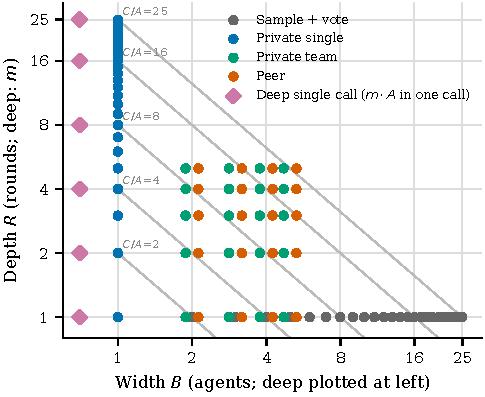
\includegraphics[width=0.55\textwidth]{figures/f1_design.pdf}
\caption{Every evaluated configuration in the width-depth plane; grey lines are iso-compute contours.
Deep calls are drawn at the left, at height $m$: one call carrying $m$ units of reasoning.}
\label{fig:design}
\end{figure}

\subsection{Estimation and multiplicity}

A configuration delivers one answer per item: plurality vote for sampling and team arms, the last
answer for private chains and deep calls. Invalid or unparseable outputs count as incorrect. All
intervals are percentile intervals from a 10,000-replicate item-clustered bootstrap, stratified by
benchmark; every configuration shares the same resample indices, so differences between configurations
are paired item by item. Macro averages weight the four benchmarks equally.

Two contrasts were frozen before collection (peer against private team at $n=4, r=4$, and the
communicate-then-private decomposition); they are quoted from the sealed contrast table. Everything else
is exploratory. In the amplification analysis every configuration is compared with independent sampling
at the same budget, and Benjamini-Hochberg control is applied within each benchmark panel.

\subsection{Limitations}

With 24 items per benchmark one item is 4.2 accuracy points, so single-benchmark differences below
roughly 15 points are not separable from noise; the macro, on 96 items, is the primary lens. Results are
from one mid-sized model and should not be assumed to transfer to larger ones. Forcing the budget is a
decode-time intervention: a forced call is not the call the model would make, and past its natural
length the model can fill the budget with repetition (Section~\ref{sec:loops}). The Math-Verify grader
timed out on {{grade_unknown_main|d}} of {{n_generations_main|d}} generations ({{grade_unknown_share|%}}),
concentrated on two items with extremely long answers; the pre-registered 5-second grading limit was kept
rather than changed after the fact, so {{checkpoint_rows_unknown|d}} of {{checkpoint_rows|d}}
configuration outcomes are unknown and are excluded pairwise from intervals (and reported as bounds in
the sealed contrasts). {{invalid_output_main|d}} generations ({{invalid_output_share|%}}) produced no
parseable final answer and score as wrong. This is a token- and dollar-accounted study, not a FLOP-matched
one.

\section{Results}

\subsection{Depth dominates at every matched budget}

Figure~\ref{fig:ladder} is the headline. On the three mathematics benchmarks the deep curve separates from
every other family by the second budget level and keeps climbing, while sampling, teams and even the
oracle ceiling of the sampling bank rise slowly.

\begin{figure}[htbp]
\centering
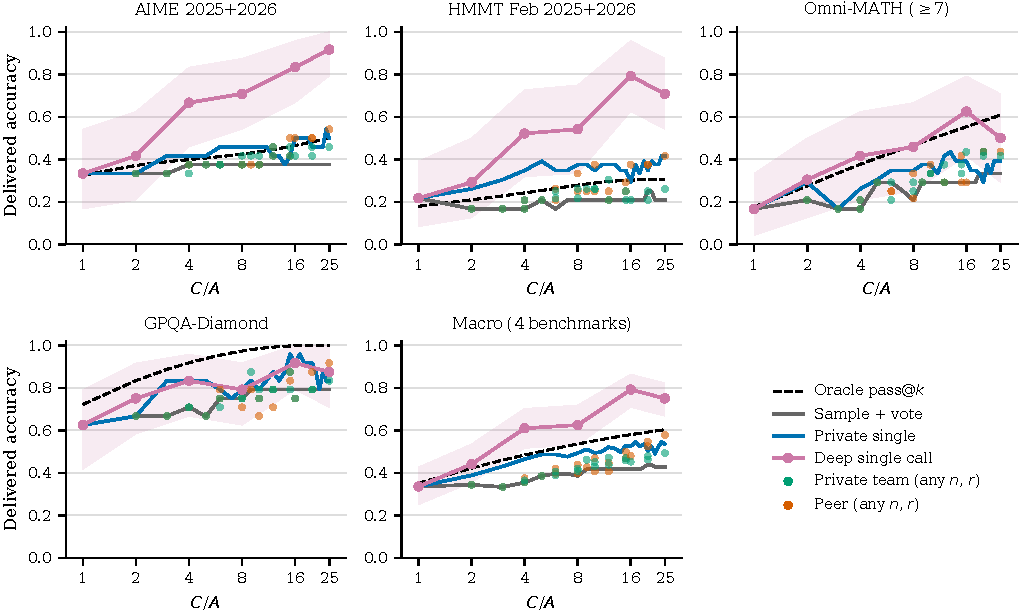
\includegraphics[width=\textwidth]{figures/f2_ladder.pdf}
\caption{Delivered accuracy against realized compute $C/A$. All points at a given $x$ spend the same number
of reasoning tokens. The dashed line is oracle pass@$k$ of the 25-sample bank, an unavailable selector.
The band is the 95\% bootstrap interval of the deep curve; dots are individual team configurations.}
\label{fig:ladder}
\end{figure}

On the macro, one sample delivers {{acc.macro.sample/1.acc|3}}. Sampling with a vote reaches
{{acc.macro.sample/16.acc|3}} at sixteen samples and {{acc.macro.sample/25.acc|3}} at twenty-five. A single
agent revising its own answer does better, {{acc.macro.private_single/16.acc|3}} after sixteen calls.
The deep call reaches {{acc.macro.deep/4.acc|3}} at $4A$, {{acc.macro.deep/8.acc|3}} at $8A$ and
{{acc.macro.deep/16.acc|3}} at $16A$ (95\% CI {{acc.macro.deep/16.lo|3}} to {{acc.macro.deep/16.hi|3}}),
the best value of any configuration in the design. At $25A$ it delivers {{acc.macro.deep/25.acc|3}}; the
difference from $16A$ is {{cross.deep25_minus_deep16.macro.pts|+1}} points (95\% CI
{{cross.deep25_minus_deep16.macro.lo|+1}} to {{cross.deep25_minus_deep16.macro.hi|+1}}), not
distinguishable from zero.

Per benchmark the pattern is sharp on competition mathematics and absent on GPQA-Diamond
(Table~\ref{tab:headline}). On AIME the deep call climbs to {{acc.aime.deep/25.acc|3}} at $25A$, while
sampling stays at {{acc.aime.sample/25.acc|3}} and the sampling oracle reaches only
{{oracle.aime.25|3}}. On HMMT deep/16 delivers {{acc.hmmt.deep/16.acc|3}} against
{{acc.hmmt.sample/16.acc|3}} for sampling. On Omni-MATH the deep call reaches {{acc.omni_math_hard.deep/16.acc|3}}
at $16A$ against {{acc.omni_math_hard.sample/16.acc|3}}. On GPQA-Diamond sampling already starts at
{{acc.gpqa_diamond.sample/1.acc|3}} and its oracle saturates near 1; the best configuration there is
{{best.gpqa_diamond.name|tt}} at {{best.gpqa_diamond.acc|3}}, and deep calls and revision chains
are statistically indistinguishable.

\begin{table}[htbp]
\centering
\small
\begin{tabular}{lrrrrrrr}
\toprule
Benchmark & pass@1 & vote@25 & oracle@25 & priv.\ 25 & best team & deep/16 & deep/25 \\
\midrule
AIME 25+26 & 0.333 & 0.375 & 0.500 & 0.500 & 0.542 & 0.833 & 0.917 \\
HMMT Feb 25+26 & 0.217 & 0.208 & 0.304 & 0.417 & 0.417 & 0.792 & 0.708 \\
Omni-MATH $\geq$7 & 0.167 & 0.333 & 0.609 & 0.391 & 0.435 & 0.625 & 0.500 \\
GPQA-Diamond & 0.625 & 0.792 & 1.000 & 0.833 & 0.917 & 0.917 & 0.875 \\
Macro (4) & 0.336 & 0.427 & 0.603 & 0.535 & 0.577 & 0.792 & 0.750 \\
\bottomrule
\end{tabular}

\caption{Delivered accuracy of reference configurations. vote@25 is sample/25; oracle@25 is pass@25 of
the same bank; priv.\ 25 is a 25-call private revision chain; best team is the best peer or private-team
configuration on that row.}
\label{tab:headline}
\end{table}

\subsection{Depth against width against revision, at equal realized compute}

Figure~\ref{fig:dvw} and Table~\ref{tab:dvw} make the comparison exact. At every budget level from $4A$
upward, on the macro, the deep call beats sampling at the same budget, beats a private revision chain of
the same total length, and the revision chain beats sampling. The margins are large: deep minus sample is
{{depth_vs_width.macro.4.deep_minus_sample.pts|+1}} points at $4A$,
{{depth_vs_width.macro.8.deep_minus_sample.pts|+1}} at $8A$, {{depth_vs_width.macro.16.deep_minus_sample.pts|+1}}
at $16A$ and {{depth_vs_width.macro.25.deep_minus_sample.pts|+1}} at $25A$, every interval excluding zero.
Deep minus revision is {{depth_vs_width.macro.16.deep_minus_private.pts|+1}} points at $16A$ (95\% CI
{{depth_vs_width.macro.16.deep_minus_private.lo|+1}} to {{depth_vs_width.macro.16.deep_minus_private.hi|+1}}).

\begin{figure}[htbp]
\centering
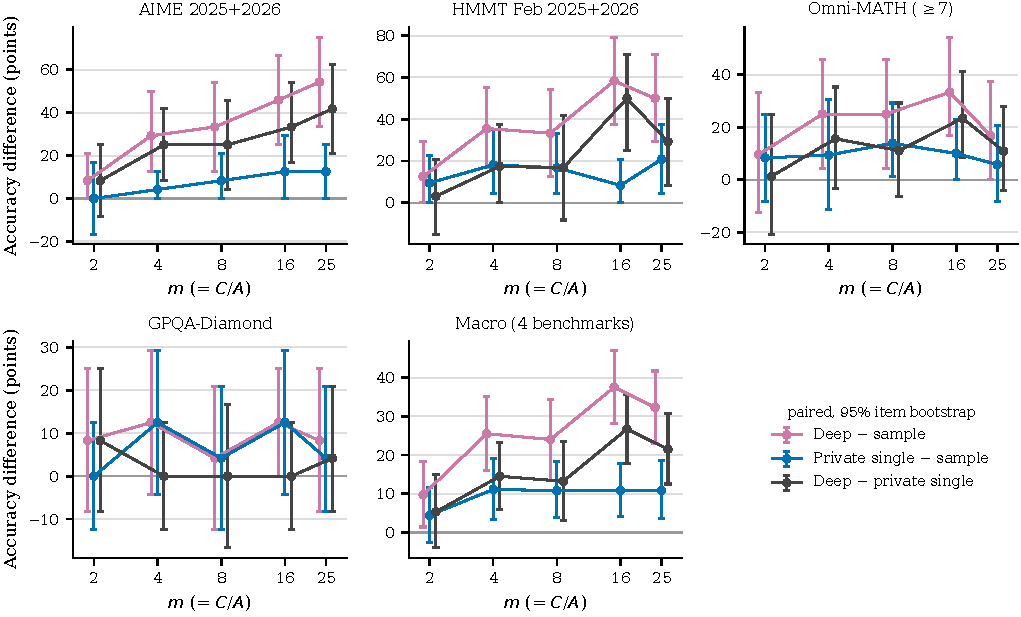
\includegraphics[width=\textwidth]{figures/f3_depth_vs_width.pdf}
\caption{Paired differences at equal realized compute $C = mA$: one deep call minus $m$ samples with a vote,
an $m$-call revision chain minus $m$ samples, and the deep call minus the revision chain. Bars are 95\%
item-clustered bootstrap intervals.}
\label{fig:dvw}
\end{figure}

\begin{table}[htbp]
\centering
\small
\begin{tabular}{rrrrrr}
\toprule
$m$ & macro deep $-$ sample & 95\% CI & deep $-$ private & 95\% CI & private $-$ sample \\ \midrule
2 & +9.7 & [+1.4, +18.2] & +5.3 & [$-$4.0, +14.9] & +4.4 \\
4 & +25.5 & [+15.9, +35.1] & +14.5 & [+5.9, +23.2] & +11.1 \\
8 & +24.0 & [+13.5, +34.4] & +13.2 & [+3.1, +23.6] & +10.8 \\
16 & +37.5 & [+28.1, +46.9] & +26.7 & [+17.7, +35.7] & +10.8 \\
25 & +32.3 & [+22.9, +41.7] & +21.5 & [+12.5, +30.8] & +10.8 \\
\bottomrule
\end{tabular}

\caption{Macro paired differences in accuracy points at equal realized compute $C = mA$.}
\label{tab:dvw}
\end{table}

The comparison also runs across budgets, and there depth wins at a fraction of the cost. A single call at
$4A$ beats twenty-five samples by {{cross.deep4_minus_sample25.macro.pts|+1}} points (95\% CI
{{cross.deep4_minus_sample25.macro.lo|+1}} to {{cross.deep4_minus_sample25.macro.hi|+1}}). A call at $8A$ is
{{cross.deep8_minus_private25.macro.pts|+1}} points above a 25-call revision chain (95\% CI
{{cross.deep8_minus_private25.macro.lo|+1}} to {{cross.deep8_minus_private25.macro.hi|+1}}, so at a third
of the compute it at least matches it). A call at $16A$
beats the best five-agent team at 25 units, \texttt{peer/5/4}, by {{cross.deep16_minus_peer54.macro.pts|+1}}
points (95\% CI {{cross.deep16_minus_peer54.macro.lo|+1}} to {{cross.deep16_minus_peer54.macro.hi|+1}}).
Per benchmark (Table~\ref{tab:dvwb}) the advantage is largest on HMMT and AIME and vanishes on GPQA-Diamond.

\begin{table}[htbp]
\centering
\small
\begin{tabular}{rlrrrr}
\toprule
$m$ & contrast & AIME & HMMT & Omni & GPQA \\ \midrule
2 & deep $-$ sample & +8.3 & +12.5 & +9.6 & +8.3 \\
2 & deep $-$ private & +8.3 & +3.1 & +1.3 & +8.3 \\
2 & private $-$ sample & +0.0 & +9.4 & +8.3 & +0.0 \\
\addlinespace
4 & deep $-$ sample & +29.2 & +35.5 & +25.0 & +12.5 \\
4 & deep $-$ private & +25.0 & +17.4 & +15.6 & +0.0 \\
4 & private $-$ sample & +4.2 & +18.1 & +9.4 & +12.5 \\
\addlinespace
8 & deep $-$ sample & +33.3 & +33.3 & +25.0 & +4.2 \\
8 & deep $-$ private & +25.0 & +16.7 & +11.1 & +0.0 \\
8 & private $-$ sample & +8.3 & +16.7 & +13.9 & +4.2 \\
\addlinespace
16 & deep $-$ sample & +45.8 & +58.3 & +33.3 & +12.5 \\
16 & deep $-$ private & +33.3 & +50.0 & +23.4 & +0.0 \\
16 & private $-$ sample & +12.5 & +8.3 & +10.0 & +12.5 \\
\addlinespace
25 & deep $-$ sample & +54.2 & +50.0 & +16.7 & +8.3 \\
25 & deep $-$ private & +41.7 & +29.2 & +10.9 & +4.2 \\
25 & private $-$ sample & +12.5 & +20.8 & +5.8 & +4.2 \\
\bottomrule
\end{tabular}

\caption{Per-benchmark paired differences in points at equal realized compute. With 24 items per benchmark
one item is 4.2 points; intervals are in \texttt{numbers.json}.}
\label{tab:dvwb}
\end{table}

\subsection{Depth reaches answers that no selector over short samples could}

In v1 the binding constraint was selection: the sampling bank contained the right answer far more often
than any vote found it. The same gap exists here, and grows with $k$: at $k=25$ oracle pass@$k$ exceeds the
vote readout by {{selection_gap_pts.macro.25|1}} macro points (Figure~\ref{fig:sel}). But the deep call
does not merely close that gap; it goes past the ceiling. deep/$m$ exceeds oracle pass@$m$ of the sampling
bank by {{deep_vs_oracle.macro.4|1}} points at $m=4$ and {{deep_vs_oracle.macro.16|1}} at $m=16$ on the
macro, and by {{deep_vs_oracle.hmmt.16|1}} points on HMMT at $m=16$. Twenty-five independent 1024-token
attempts at an HMMT problem contain a correct answer on {{oracle.hmmt.25|3}} of items; one 16,384-token
attempt is correct on {{acc.hmmt.deep/16.acc|3}}. The limit of a short sample is not that the right answer is
hard to pick out; it is that a short sample usually does not produce it at all.

\begin{figure}[htbp]
\centering
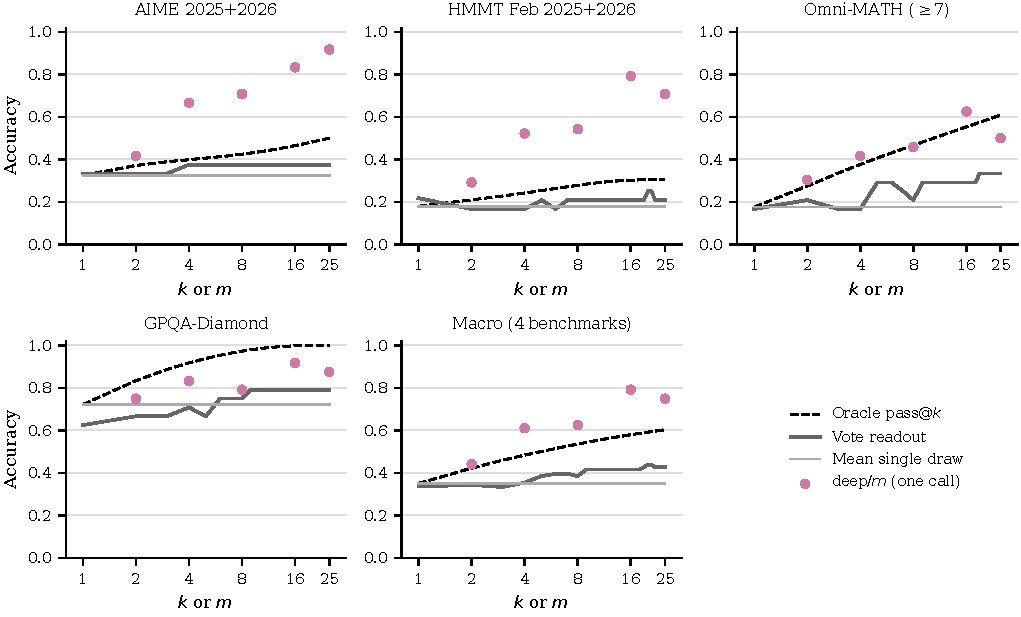
\includegraphics[width=\textwidth]{figures/f6_selection.pdf}
\caption{The sampling bank at $A=1024$: oracle pass@$k$, the vote readout and the mean single draw, with
the deep call at $m$ times the budget overlaid. Points above the dashed line are beyond anything a
selector over $k$ short samples could deliver.}
\label{fig:sel}
\end{figure}

The exception is GPQA-Diamond, where the sampling oracle reaches {{oracle.gpqa_diamond.25|3}} and the deep
call stays below it ({{deep_vs_oracle.gpqa_diamond.16|+1}} points at $m=16$). A multiple-choice question
whose answer a short sample often reaches is a selection problem, as in v1; a competition problem whose
answer a short sample rarely reaches is a depth problem.

\subsection{The amplification matrix}

Figure~\ref{fig:matrix} compares every allocation with independent sampling at the same budget. On the macro,
{{iso.macro.n_sig_pos|d}} of {{iso.macro.n_tests|d}} comparisons are significantly positive after
Benjamini-Hochberg control and {{iso.macro.n_sig_neg|d}} are significantly negative. By family:
{{iso.macro.by_family.deep.n_sig_pos|d}} of {{iso.macro.by_family.deep.n|d}} deep calls (mean
{{iso.macro.by_family.deep.mean_delta_pts|+1}} points), {{iso.macro.by_family.private_single.n_sig_pos|d}} of
{{iso.macro.by_family.private_single.n|d}} revision chains (mean {{iso.macro.by_family.private_single.mean_delta_pts|+1}}),
{{iso.macro.by_family.peer.n_sig_pos|d}} of {{iso.macro.by_family.peer.n|d}} peer teams (mean
{{iso.macro.by_family.peer.mean_delta_pts|+1}}) and {{iso.macro.by_family.private_team.n_sig_pos|d}} of
{{iso.macro.by_family.private_team.n|d}} private teams (mean {{iso.macro.by_family.private_team.mean_delta_pts|+1}}).
No allocation does significantly worse than sampling. This is the opposite of v1, where none of 70
per-benchmark comparisons survived correction.

\begin{figure}[htbp]
\centering
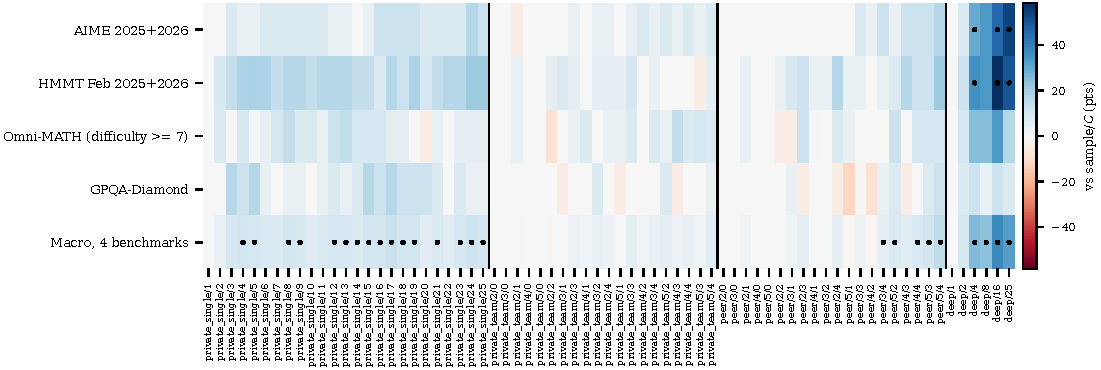
\includegraphics[width=\textwidth]{figures/f5_amplification_matrix.pdf}
\caption{Each allocation minus independent sampling at the same budget, in accuracy points. Dots mark
cells significant after Benjamini-Hochberg control within the row. Columns are grouped by family.}
\label{fig:matrix}
\end{figure}

\subsection{Repetition inside forced calls}
\label{sec:loops}

Forcing a model past the point where it would stop can produce degenerate repetition. We detect a loop as
the first 3,000-character window of the reasoning whose zlib compression ratio falls below 0.1 and count
the reasoning before it as effective depth (Table~\ref{tab:loops}, Figure~\ref{fig:loops}). No 1024-token
call looped. The share of deep calls that loop rises to {{effective_depth.16.looped_share|3}} at $16A$ and is
{{effective_depth.25.looped_share|3}} at $25A$; on average {{effective_depth.16.eff_fraction_mean|3}} of a
$16A$ call's tokens precede any loop.

\begin{table}[htbp]
\centering
\small
\begin{tabular}{rrrrrr}
\toprule
deep/$m$ & reasoning tokens & calls looping & mean effective tokens & effective share & loop onset (median) \\ \midrule
2 & 2,048 & 0.000 & 2,048 & 1.000 & -- \\
4 & 4,096 & 0.052 & 3,950 & 0.965 & 1,243 \\
8 & 8,192 & 0.146 & 7,554 & 0.922 & 3,140 \\
16 & 16,384 & 0.281 & 13,833 & 0.844 & 7,190 \\
25 & 25,600 & 0.208 & 22,319 & 0.872 & 6,701 \\
\bottomrule
\end{tabular}

\caption{Deep calls by forced length. Effective tokens are reasoning before loop onset (all of it for calls
that never loop). Loop onset is the median over looping calls.}
\label{tab:loops}
\end{table}

The loops are not what they appear. A looping call is \emph{more} likely to be correct, not less:
{{deep_acc_by_loop.16.looped|3}} against {{deep_acc_by_loop.16.clean|3}} at $16A$, and
{{deep_acc_by_loop.25.looped|3}} against {{deep_acc_by_loop.25.clean|3}} at $25A$. A call loops when it has
already worked the problem out and has nothing left to do but restate it; the calls that still use the
whole budget productively are the hard ones. The dip from $16A$ to $25A$ on HMMT and Omni-MATH, not
significant on 24 items each, is consistent with this: past the length at which most problems are solved,
extra forced tokens add little and occasionally disturb a finished answer.

\begin{figure}[htbp]
\centering
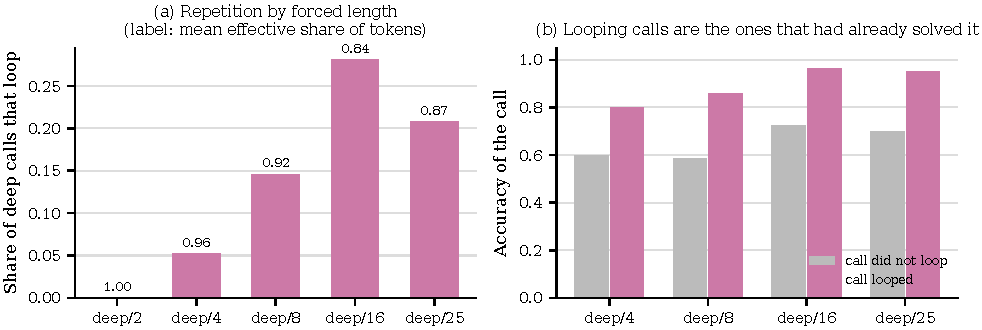
\includegraphics[width=0.85\textwidth]{figures/f8_effective_depth.pdf}
\caption{(a) Share of deep calls whose reasoning degenerates into repetition, labelled with the mean share of
tokens before loop onset. (b) Accuracy of deep calls that looped against those that did not.}
\label{fig:loops}
\end{figure}

\subsection{The cost of letting agents talk}

In v1, peer exposure destroyed accuracy, increasingly with rounds. Here it helps slightly on average:
across the 16 team shapes peer minus private team averages {{comm.mean_pts|+1}} macro points, positive in
{{comm.n_pos|d}} of {{comm.n_cells|d}} cells (Figure~\ref{fig:comm}); at five agents and four rounds it is
{{comm.cell_5_4.delta|+1}} points (95\% CI {{comm.cell_5_4.lo|+1}} to {{comm.cell_5_4.hi|+1}}). The frozen
primary contrast at $n=4$, $r=4$ is {{primary.primary_i_peer_vs_private_team_n4_r4.estimate_pts|+1}} points
on {{primary.primary_i_peer_vs_private_team_n4_r4.n_complete|d}} of
{{primary.primary_i_peer_vs_private_team_n4_r4.n|d}} complete items (sealed bounds
{{primary.primary_i_peer_vs_private_team_n4_r4.bound_lo_pts|+1}} to
{{primary.primary_i_peer_vs_private_team_n4_r4.bound_hi_pts|+1}}); because one item carries an unknown grade
the sealed table withholds a Holm $p$-value, and the known-items paired interval is
{{primary_peer_known.lo|+1}} to {{primary_peer_known.hi|+1}} points (Table~\ref{tab:primary}). The gain is
concentrated on HMMT. Either way, every team configuration is far below a single deep call at comparable
or lower cost.

\begin{figure}[htbp]
\centering
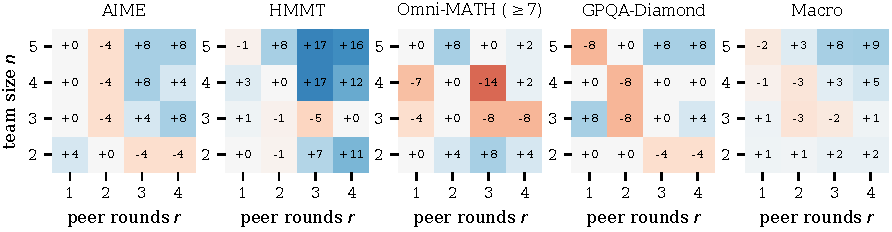
\includegraphics[width=\textwidth]{figures/f7_communication.pdf}
\caption{Peer minus private team, in accuracy points, by team size and number of peer rounds. Both arms
spend identical compute; only exposure to peers differs.}
\label{fig:comm}
\end{figure}

\begin{table}[htbp]
\centering
\small
\begin{tabular}{lrrrr}
\toprule
Contrast (sealed, frozen before collection) & estimate (pts) & bounds (pts) & complete & status \\ \midrule
(i) peer/4/4 $-$ private\_team/4/4 & +4.2 & [+4.2, +5.2] & 95/96 & partial \\
(ii) CP gain $-$ private-team gain, $h$=3 & +1.1 & [+0.0, +2.1] & 94/96 & partial \\
\bottomrule
\end{tabular}

\caption{The two contrasts frozen before collection, as sealed. ``partial'' means some items carry an
unknown grade: the estimate is over complete items and the bounds fix every unknown term at its extremes.}
\label{tab:primary}
\end{table}

\subsection{What this costs in dollars}

Realized compute and dollars are close to proportional in this design, but not exactly: a deep call pays
for its long reasoning once, while a revision chain or a team re-reads prompts and candidate packets on
every call. The accuracy-per-dollar frontier (Figure~\ref{fig:dollars}) consists entirely of deep calls:
\texttt{deep/16} delivers {{acc.macro.deep/16.acc|3}} at {{cost_usd.deep/16|3}} dollars per item, while
\texttt{sample/25} delivers {{acc.macro.sample/25.acc|3}} at {{cost_usd.sample/25|3}} and \texttt{peer/5/4}
delivers {{acc.macro.peer/5/4.acc|3}} at {{cost_usd.peer/5/4|3}}.

\begin{figure}[htbp]
\centering
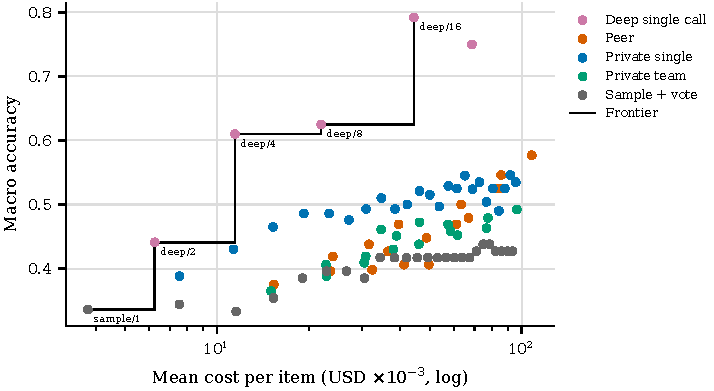
\includegraphics[width=0.7\textwidth]{figures/f9_dollars.pdf}
\caption{Macro accuracy against mean generation cost per item (all calls of the configuration, both THINK
and ANSWER). The step line is the frontier of configurations not dominated on both axes.}
\label{fig:dollars}
\end{figure}

\subsection{Robustness}

The two providers served disjoint items, so provider is a covariate, not a paired contrast. The depth
advantage appears on both (Figure~\ref{fig:rob}): deep/16 minus sample/16 is
{{robustness.mancer.deep_vs_sample.16.delta_pts|+1}} points on Mancer's {{robustness.mancer.items|d}} items
and {{robustness.parasail.deep_vs_sample.16.delta_pts|+1}} on Parasail's {{robustness.parasail.items|d}},
although the two item sets differ in difficulty (pass@1 {{robustness.mancer.pass1|3}} and
{{robustness.parasail.pass1|3}}). Unknown grades affect {{checkpoint_rows_unknown|d}} configuration outcomes
on two items; each item is about one macro point, so they cannot move any macro comparison above by more than about two points.

\begin{figure}[htbp]
\centering
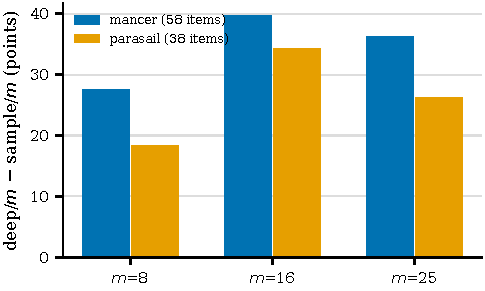
\includegraphics[width=0.5\textwidth]{figures/f10_robustness.pdf}
\caption{deep/$m$ minus sample/$m$ within each provider's items.}
\label{fig:rob}
\end{figure}

\section{Interpretation}

v1 concluded that the binding constraint was selection and that allocation shape barely mattered. With the
budget actually spent, that conclusion is overturned on hard reasoning problems. The dominant lever is the
length of a single uninterrupted chain of thought. Sixteen short calls, whether sampled independently,
arranged into teams or allowed to debate, do not add up to one long one: their pool reaches the right
answer far less often than a single call of the same total length, so no amount of voting, verification or
communication can recover the difference.

On the macro, the ordering at equal realized compute is: one deep call, then one agent revising its own
answer serially, then teams, then independent samples with a vote (mean advantage over sampling
{{iso.macro.by_family.deep.mean_delta_pts|+1}}, {{iso.macro.by_family.private_single.mean_delta_pts|+1}},
{{iso.macro.by_family.peer.mean_delta_pts|+1}} for peer and {{iso.macro.by_family.private_team.mean_delta_pts|+1}}
for private teams). Per benchmark the middle of the ordering is noisy (on Omni-MATH the best non-deep
configuration is a private team), but depth is first on all three mathematics benchmarks. It is an ordering by how much of the compute goes into a single continuous line of reasoning. Serial
revision keeps some of that continuity (each call reads the previous answer) but restarts the reasoning
at every call; teams split it further; independent samples discard it entirely.

Two boundaries limit the claim. First, the regime: at $A=1024$ every short call is badly truncated on
these problems, whose natural reasoning runs to thousands of tokens. When a single call already has
enough room, as on easy problems in our pilots, forcing it longer buys repetition rather than accuracy, and
the problem becomes one of selection again, as on GPQA-Diamond here. The relevant quantity is the budget
relative to the length of reasoning the problem requires. Second, the model: this is one 27B model, and the
ability to use a long budget productively is a property of the model's training.

\section{What to do with this}

\begin{enumerate}
\item \textbf{Spend on depth before width when a single call is budget-limited.} If a model's natural
reasoning on a task is longer than the per-call budget, raising the per-call budget dominates adding calls.
On this benchmark mix a call at $4A$ beat twenty-five calls at $A$.
\item \textbf{Measure natural length first.} The forcing mechanism and the calibration above give that
number cheaply; depth pays up to roughly the natural length and loses its value beyond it.
\item \textbf{Keep serial revision as the second lever} when a single call cannot be made longer (for
example, a hard context or latency limit per call): it is above sampling at every budget of three calls or
more, by {{iso.macro.by_family.private_single.mean_delta_pts|1}} points on average.
\item \textbf{Treat selection as the lever only where short samples already reach the answer} (the GPQA
regime), which is where v1's verification prescription still applies.
\end{enumerate}

\appendix
\section{Run facts}

Total generation cost {{spend_all_usd|$}} (accepted generations), of which the main run
{{spend_main_usd|$}}; OpenRouter key usage over the study window {{ledger.key_delta_usd|$}}. The ledger
charged {{ledger.charged_total_usd|$}}, above key usage because {{ledger.charged_max_usd|$}} of ambiguous
attempts were conservatively charged at their full reservation; its invariant checks recorded
{{ledger.invariant_violations|d}} violations. Canary {{ledger.canary_settled_usd|$}}, calibration
{{ledger.calibration_settled_usd|$}}, pilot {{ledger.pilot_settled_usd|$}}. The main run dispatched
{{n_generations_main|d}} generation nodes, each two HTTP calls, over two concurrent provider shards in
about 1.6 hours; median visible answer length was {{answer_tokens_median|d}} tokens. All pre-registered gates
passed, with two notes. The canary's check of the ledger against provider usage first failed because both
shards bill one key concurrently, so each shard's usage window contained the other's spend; it was
re-evaluated over the union of the windows against the sum of both ledgers, and passed. And there were two
owner-accepted exceptions on the Mancer pilot (AIME invalid finals at 94.4\% against 95\%,
and a forecast above that shard's proportional budget slice, resolved by re-splitting the \$95 cap).
Sealed tables, the merge manifest and every figure and number in this report are regenerated by
\texttt{build.sh} from the run directory.

\end{document}
